\section{Investigating more Complex Geometries Numerically}

It is often practical in mathematics to find alternative ways of modelling otherwise complicated systems in terms of other more abstract models. Let us take for example something already brought up in this paper as an example of the application of Lagrangian Mechanics: the Simple Pendulum. 

\vspace{1em}
Consider the case where the golf course surface is a perfectly hemispherical well of radius $a$ centered at the origin, described biparametrically (in the best way I could figure out) by the height field
\begin{equation}
	h(q^1, q^2) = -a\sqrt{\frac{1-\frac{(q^1)^2+(q^2)^2}{a^2}+\sqrt{\left(1-\frac{(q^1)^2+(q^2)^2}{a^2}\right)^2+\varepsilon^2}}{2}},
\end{equation}
where the hemispherical well has radius $a$ and $\varepsilon\ll 1$ or $\approx 0$ describing the hemisphere edge smoothness as it transitions to a flat plane. As previously discussed, the holonomic constraint $q^3 = h(q^1, q^2)$ restricts the ball to move along the hemisphere's surface. In this geometry, the equations of motion derived previously reduce precisely to those governing a 3D simple pendulum: the ball's position is always at a fixed distance $a$ from the origin, and its dynamics are determined by the interplay of gravity and the surface's curvature. This equivalence demonstrates that the golf ball model is not limited to mini-golf scenarios, but rather encodes the dynamics of a wide class of physical systems. The same formalism describes the motion of a pendulum, a particle on a sphere, or even planetary orbits under certain constraints. Thus, by analyzing the forced geodesic equations for arbitrary surfaces, we gain insight into the behavior of many seemingly different systems, unified by the underlying mathematics of constrained motion. Let us take a qualitative look at the dynamics of the golf ball on such a hemispherical surface when let to move around with some arbitrary initial velocity and position.


\begin{figure}[H]
	\centering
	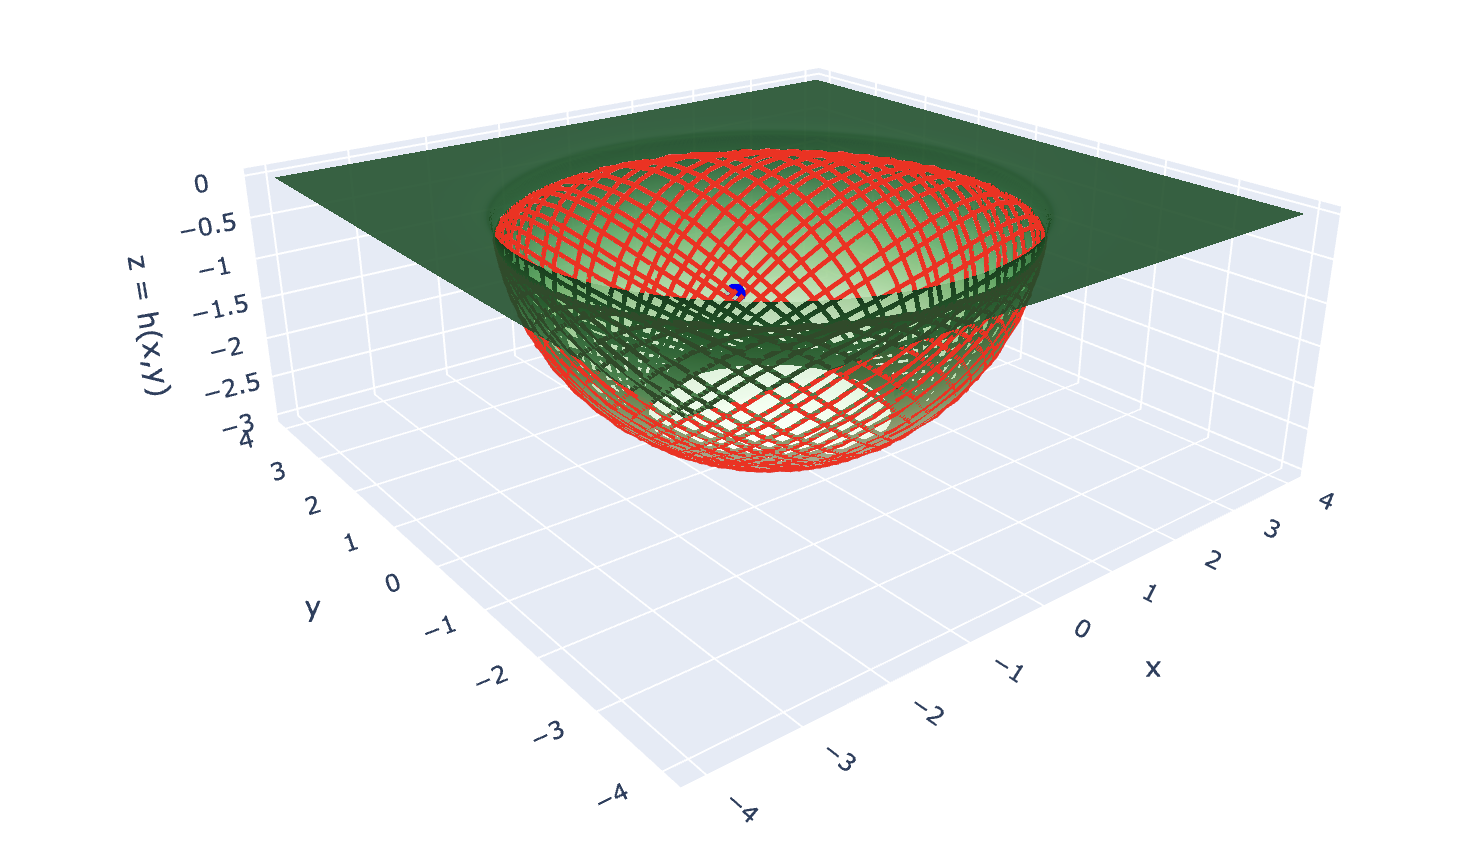
\includegraphics[width=0.55\textwidth]{assets/pend_course.png}
	\caption{Diagram demonstrating the trajectory of a golf ball confined to a hemispherical well golf course. It's dynamics exactly mimic that of a simple pendulum!}
	\label{fig:course3}
\end{figure}

Amazing! The dynamics of \ref{fig:course3} exactly mimic that of the bob of a simple 3D pendulum. Notice the beautiful patterns that it traces as it evolves through its trajectory. Below is a top down image for a more clear vizualization of the clear pattern.


\begin{figure}[H]
	\centering
	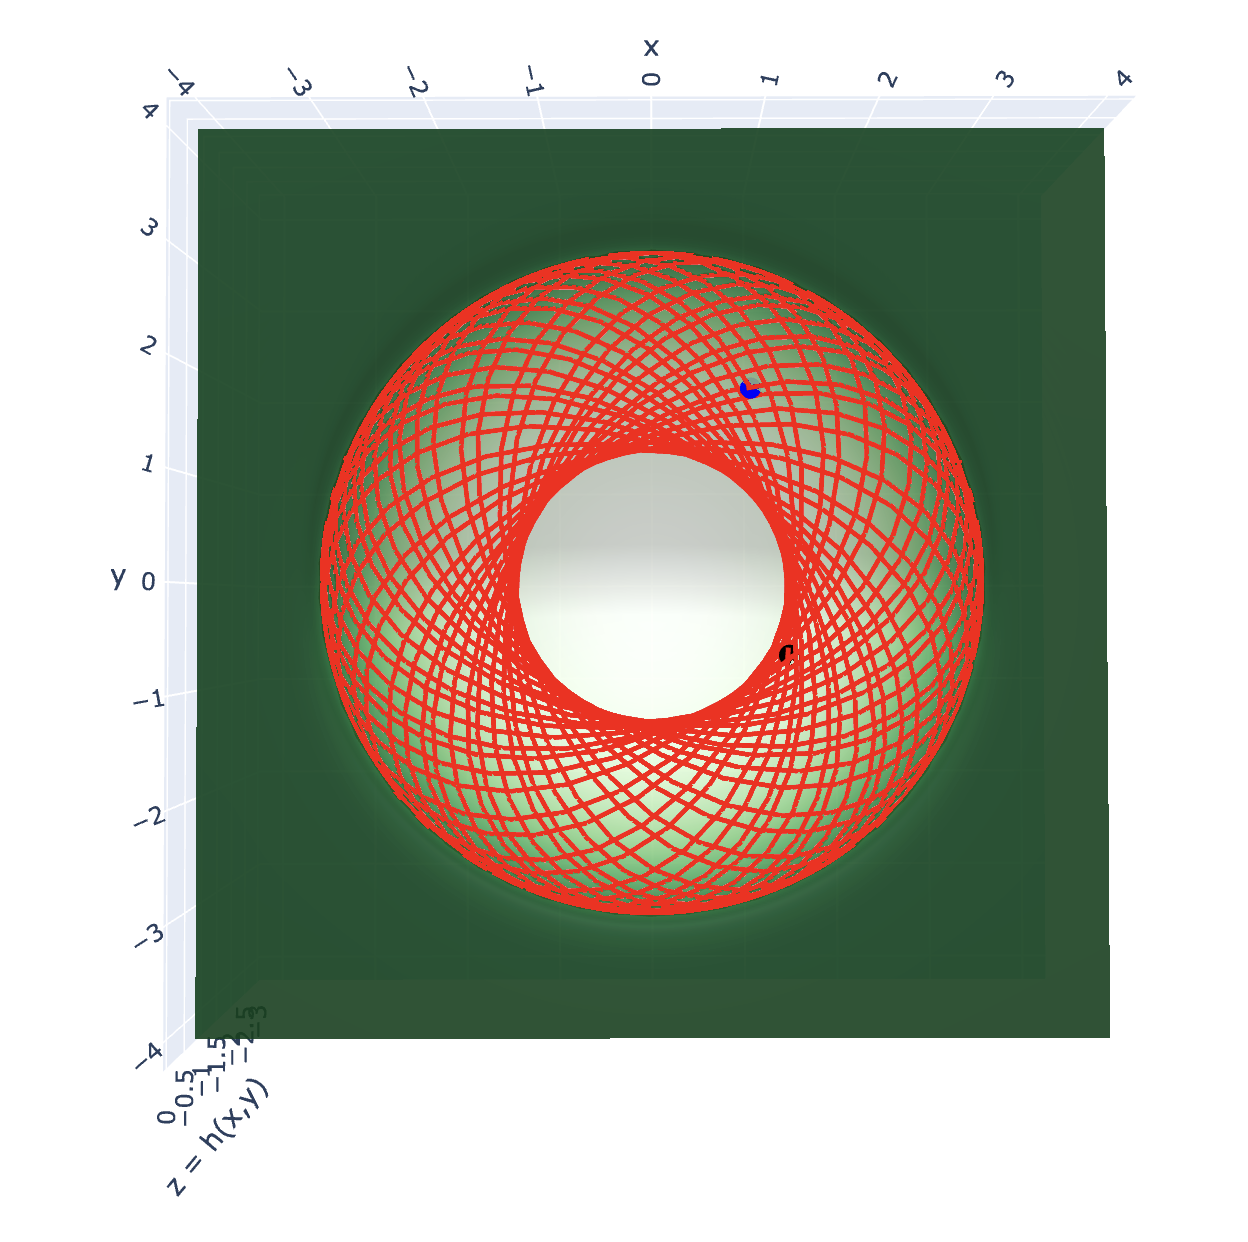
\includegraphics[width=0.3\textwidth]{assets/top_pend_course.png}
	\caption{Top down image of the hemispherical course's golf ball trajectory}
	\label{fig:cours4}
\end{figure}

